\documentclass{article}

\usepackage{arxiv}

\usepackage[utf8]{inputenc} % allow utf-8 input
\usepackage[T1]{fontenc}    % use 8-bit T1 fonts
\usepackage{hyperref}       % hyperlinks
\usepackage{url}            % simple URL typesetting
\usepackage{booktabs}       % professional-quality tables
\usepackage{amsfonts}       % blackboard math symbols
\usepackage{nicefrac}       % compact symbols for 1/2, etc.
\usepackage{microtype}      % microtypography
\usepackage{lipsum}
\usepackage{indentfirst}
\usepackage{graphicx}
\graphicspath{ {./images/} }
\usepackage{physics}
\usepackage{amsmath}
\DeclareMathOperator*{\argmin}{\arg\!\min}
\DeclareMathOperator*{\argmax}{\arg\!\max}
\usepackage{bm}
\usepackage{bbold}
\newcommand{\bd}{\textbf}
\usepackage[compact]{titlesec}  
\usepackage{float}
\usepackage{amsmath}
\usepackage{listings}
\usepackage{listings}
\usepackage{subfigure}
\usepackage{xcolor}

\definecolor{codegreen}{rgb}{0,0.6,0}
\definecolor{codegray}{rgb}{0.5,0.5,0.5}
\definecolor{codepurple}{rgb}{0.58,0,0.82}
\definecolor{backcolour}{rgb}{0.95,0.95,0.92}

\lstdefinestyle{mystyle}{
    backgroundcolor=\color{backcolour},   
    commentstyle=\color{codegreen},
    keywordstyle=\color{magenta},
    numberstyle=\tiny\color{codegray},
    stringstyle=\color{codepurple},
    basicstyle=\ttfamily\footnotesize,
    breakatwhitespace=false,         
    breaklines=true,                 
    captionpos=b,                    
    keepspaces=true,                 
    numbers=left,                    
    numbersep=5pt,                  
    showspaces=false,                
    showstringspaces=false,
    showtabs=false,                  
    tabsize=2
}

\lstset{style=mystyle}

\title{The Data Open: Using Machine Learning Methods to Analyze Titles and Predict User Behavior}
\author{
  Sharan Sahu\\
  UC Berkeley\\
  Berkeley, CA\\
  \texttt{ssahu01@berkeley.edu}
  %% examples of more authors
   \And
 Darsh Balani \\
  UC Berkeley\\
  Berkeley, CA\\
  \texttt{dbalani2002@gmail.com}
  %% \AND
  %% Coauthor \\
  %% Affiliation \\
  %% Address \\
  %% \texttt{email} \\
  %% \And
  %% Coauthor \\
  %% Affiliation \\
  %% Address \\
  %% \texttt{email} \\
  %% \And
  %% Coauthor \\
  %% Affiliation \\
  %% Address \\
  %% \texttt{email} \\
}

\begin{document}
\maketitle

\begin{abstract}
In a world dominated by technology and social media, it is important to understand how to capture ones attention and retain them as users. On average, media and entertainment have an average of 43\% retention rate in 30 days and 24\% in 90 days. With this in mind, we posed the following question in analyzing the data set: how do the headline and shared text impact the click to impression ratio and whether a package is a winner or not? Understanding the impact of headline and shared text can allow social media companies to understand what types of headlines are pertinent with their users and can increase traffic to their website or app. In this paper, we will show that both the headline and shared text impact the click to impression ratio,  page views,  and retention.
\end{abstract}

\section{Technical Exposition}

\subsection{Initial Data Exploration and Cleaning}

\setlength{\parindent}{10pt}
After looking through the different .csv data files, we decided that the packages.csv file would provide us with the most relevant data for our problem statement. In the packages file, we explored all of the columns to see which ones would impact clicks the most. We decided that the headline and share\_text columns were the best ones to use because these two features are some of the first things that a reader sees before they click on an article, whether the reader was scrolling through the website or got sent an article by a friend.  There were some basic variables in these columns that could easily be extracted into features for the models. For example, we used the number of characters, number of words, and average word length (in characters) from both the headline and shared text as model features. We also calculated the number of capitalized characters and number of specified symbols (!,   ?, *).  However, we felt like these attributes did not paint a big enough picture of our data. So, we decided to dip our toes in NLP in order to add features that were based on the individual words of the headline and shared text. More specifically, we wanted to see if and how “clickbait words” affected the click to impression ratio and whether or not the package was a winner.  After exploring the package data, we discovered that Upworthy is a website that contains many clickbait-like articles, similar to Buzzfeed. So, we defined “clickbait words” as the most used words, not including prepositions and basic nouns used for sentence structure.  We began by extracting the words from both the headline and shared text in order to clean the data. The individual words need to be cleaned, so we removed punctuation, capitalization, digits, and special characters from the data. After this, we used the nlkt library for stemming and lemmatization in order to handle cases where there exist multiple forms of the same word. We used stemming in order to remove the suffix from the words, then used lemmatization in order to group equivalent roots together.  We also had to remove individual words, such as prepositions, pronouns, conjunctions, and basic nouns used for sentence structure, as these stop words have very little meaning, but are required by English grammar. We took the default stop words from the nlkt library and added custom words based on our observations of the data.  After cleaning, we can get the count of these words. Below are the word clouds for the most used words from the headline and shared text, respectively. \par
\begin{figure}[h]
\centering
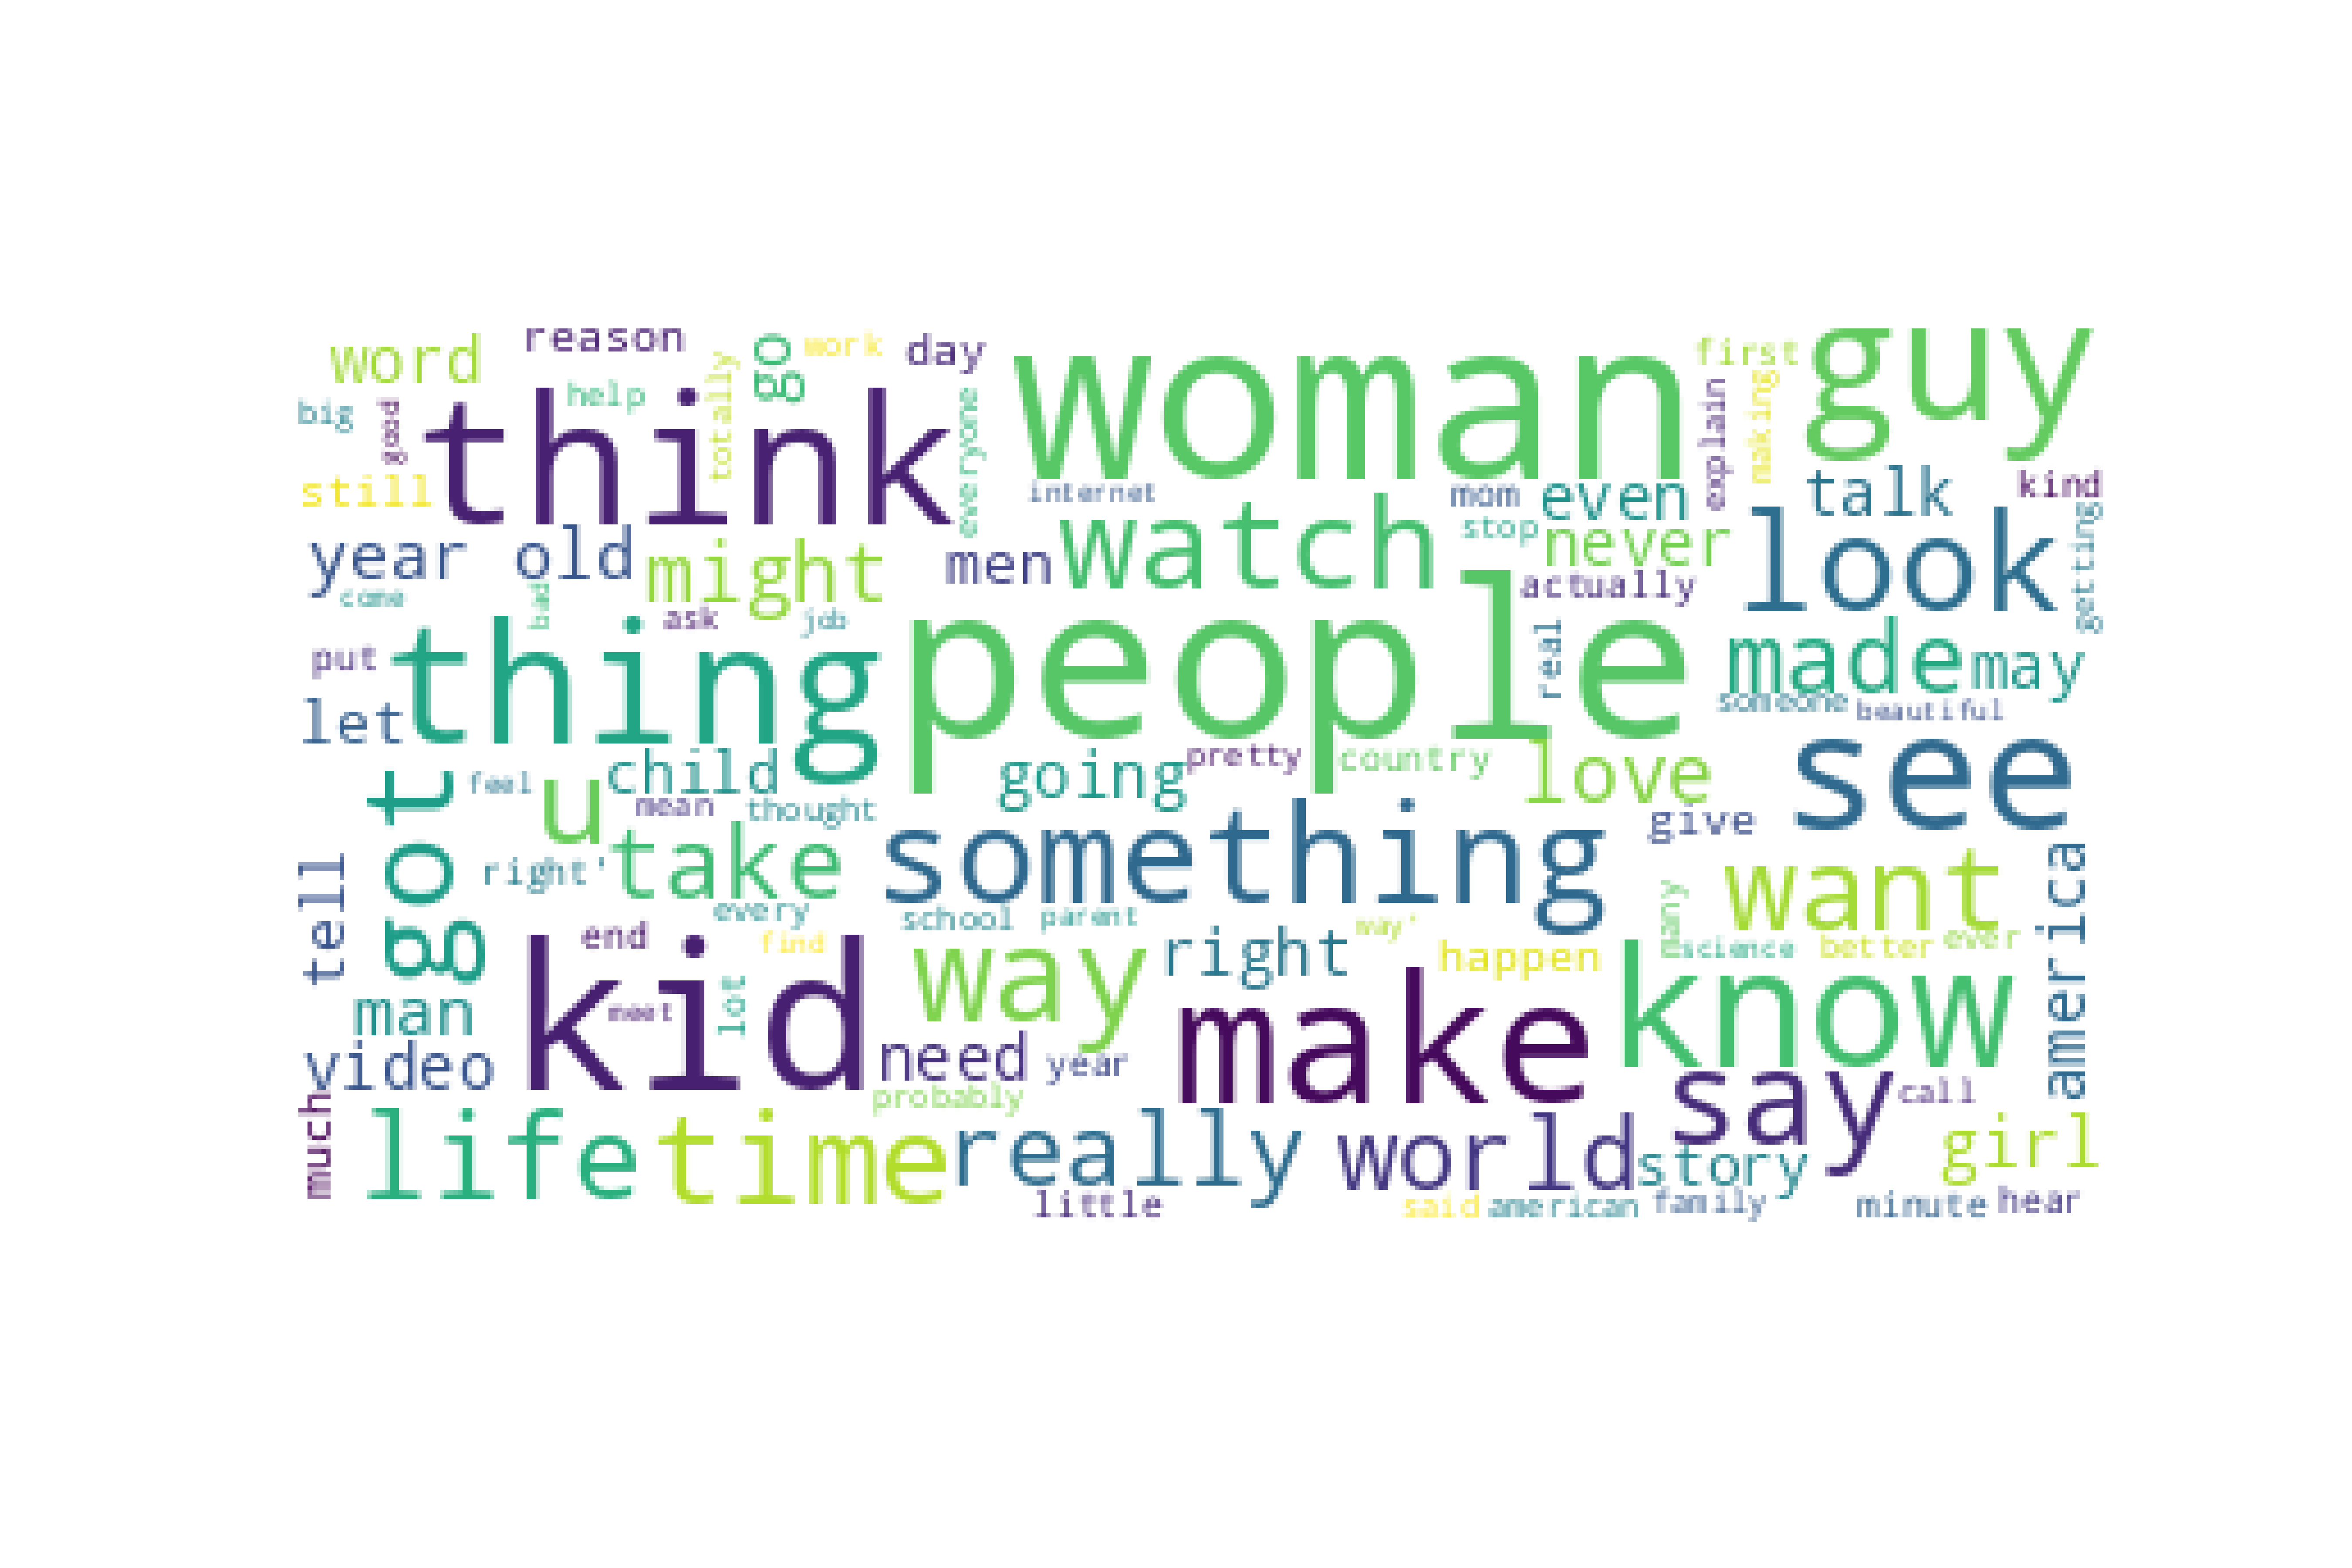
\includegraphics[scale=.3]{word1.png}
\caption{Shared\_Text Text After Pre Processing}
\end{figure} 
\begin{figure}[h]
\centering
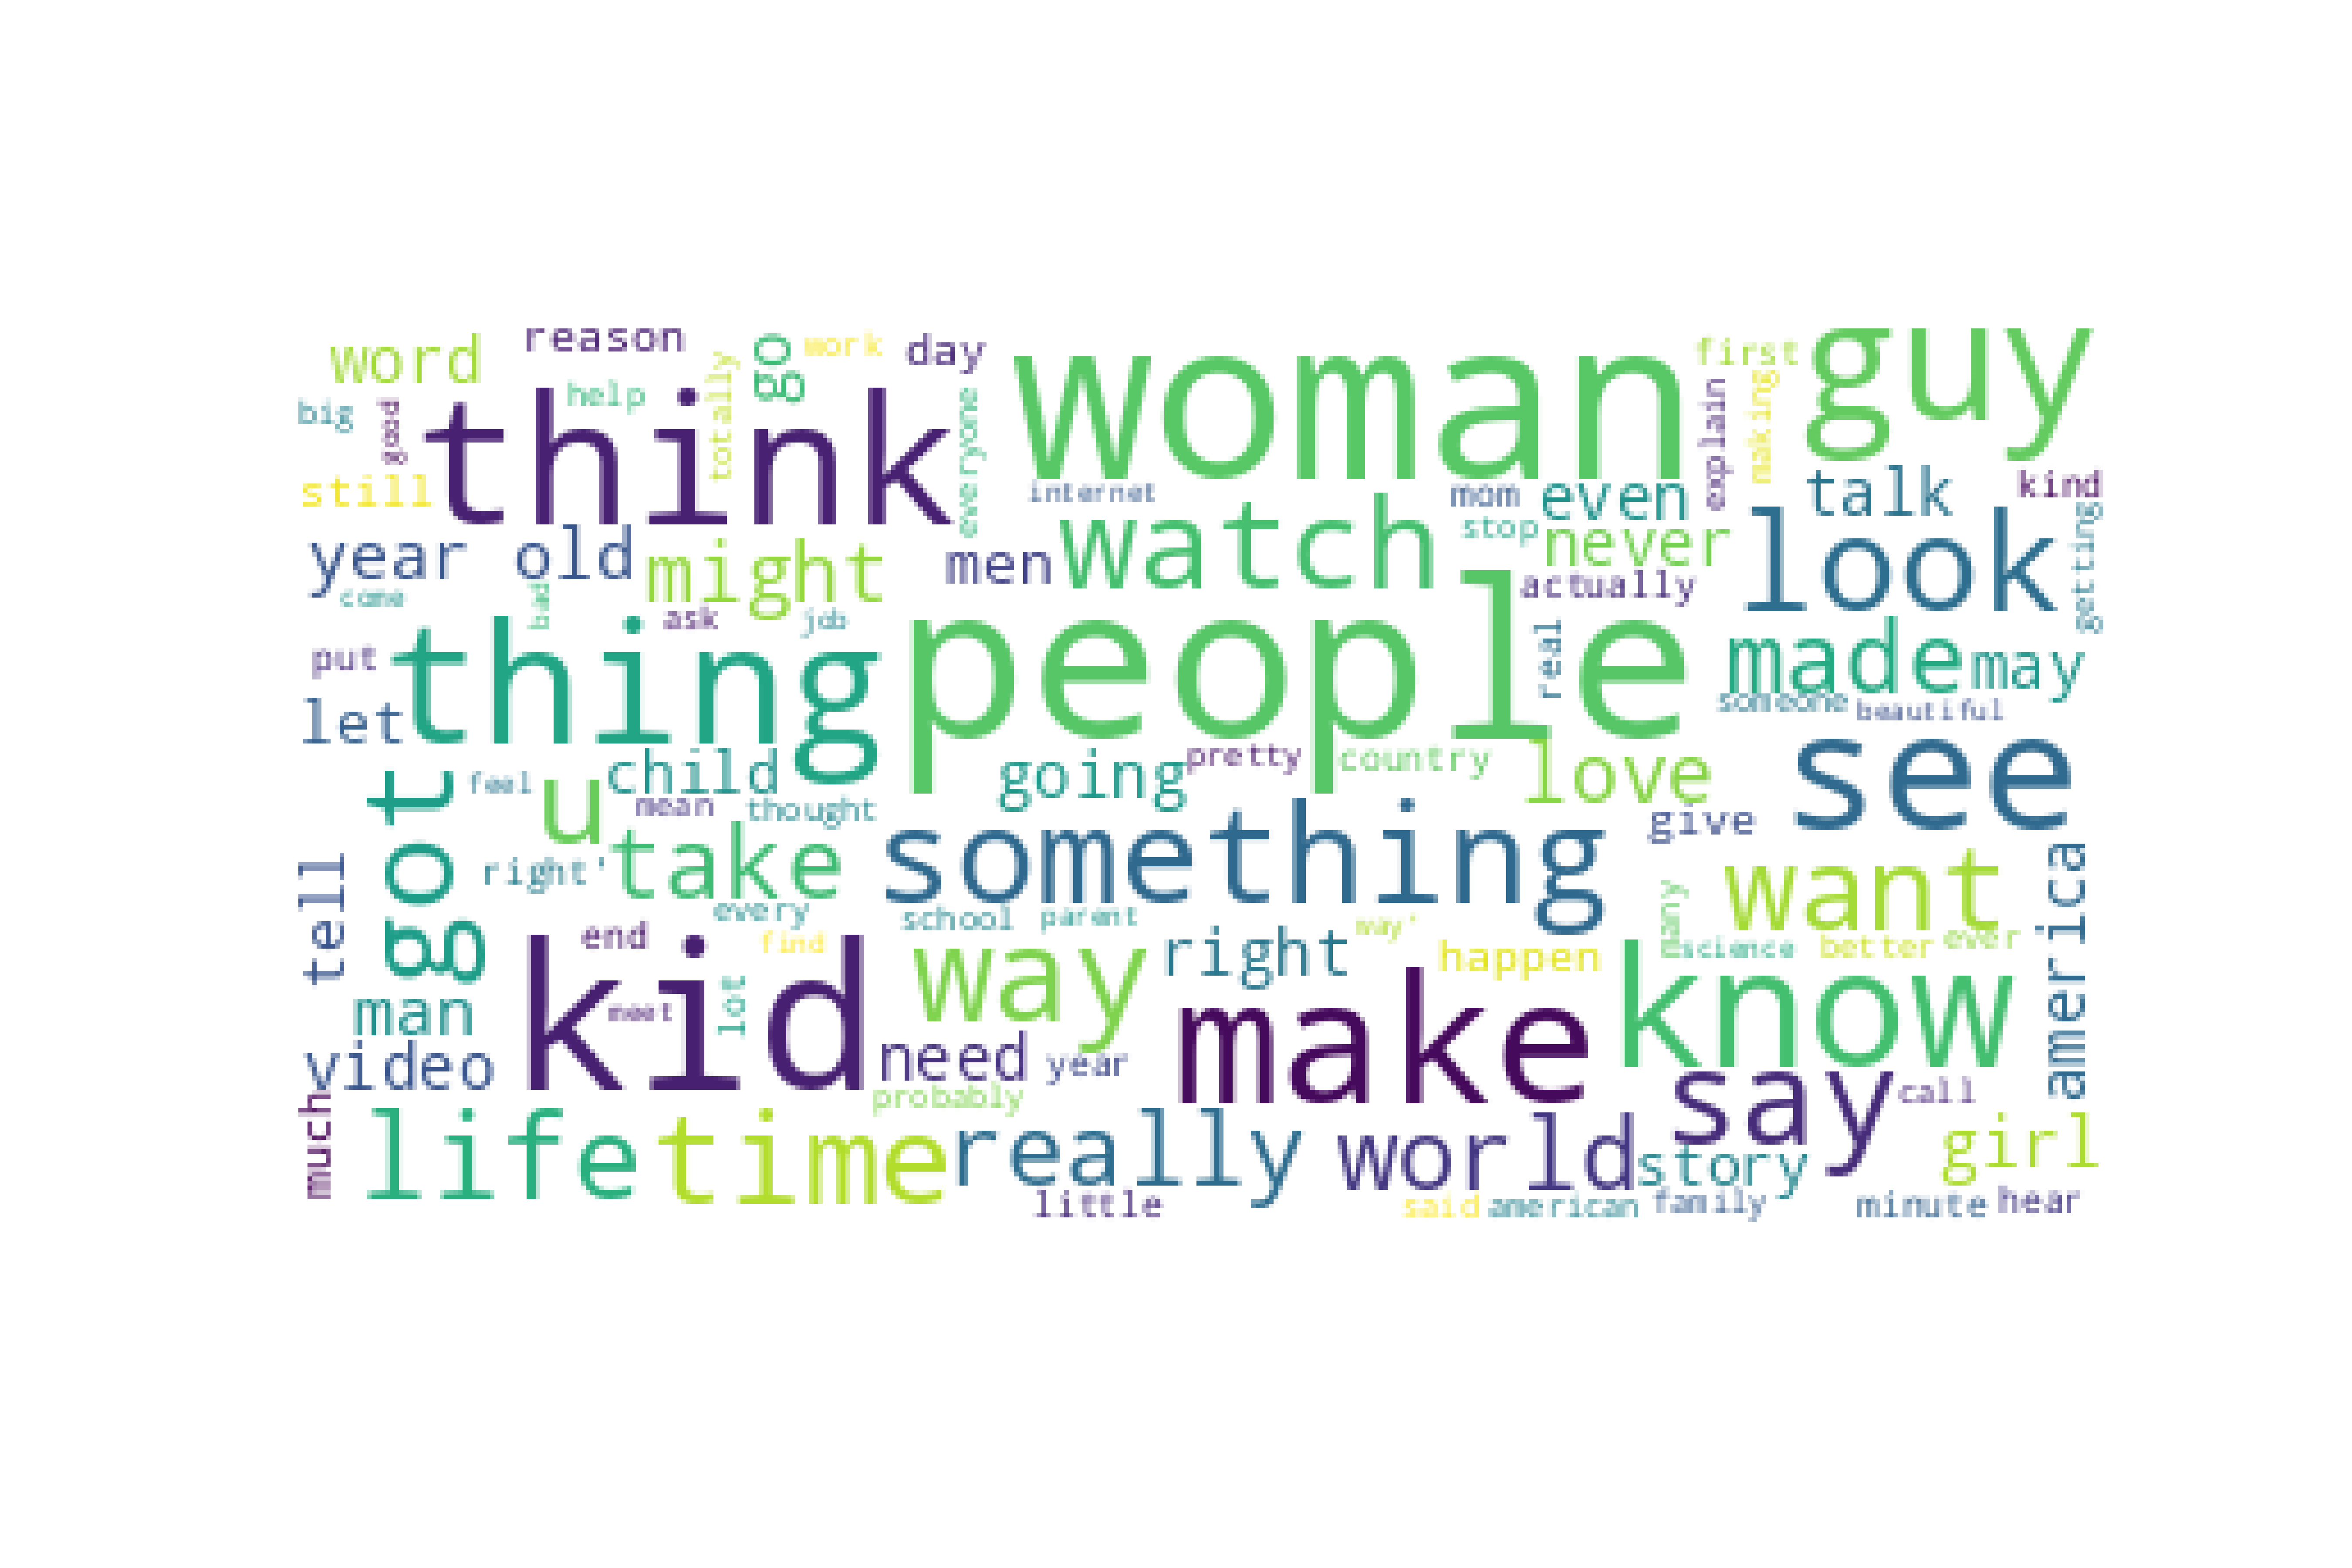
\includegraphics[scale=.3]{word1.png}
\caption{Overview Of Supervised Learning}
\end{figure} 

\subsection{Creating The NLP Model}

\setlength{\parindent}{10pt}

Now that our data has been pre processed with lematization, stemming, and the removing of extraneous string features, we can begin discussing how we set up our NLP model.  After exploring the package data, we discovered that Upworthy is a website that contains many clickbait-like articles, similar to Buzzfeed. So, we defined “clickbait words” as the most used words, not including prepositions and basic nouns used for sentence structure.  From here, we needed to convert these words into something interpretable using our NLP model. Thus, we utilized Tokenization and Vectorization for converting the continuous text into a list of words and then converted the list of words into a matrix of integers.  We decided to use both 1-word and 2-word phrases as part of the model, so we counted by both 1-word and 2-word phrases.  After looking at the data, we decided to use the twenty most used 1-word and 2-word phrases for our model.  Below are graphs of the most used twenty 1-word and 2-word phrases from the headline and shared text, respectively. 

\begin{figure}[h]
\centering
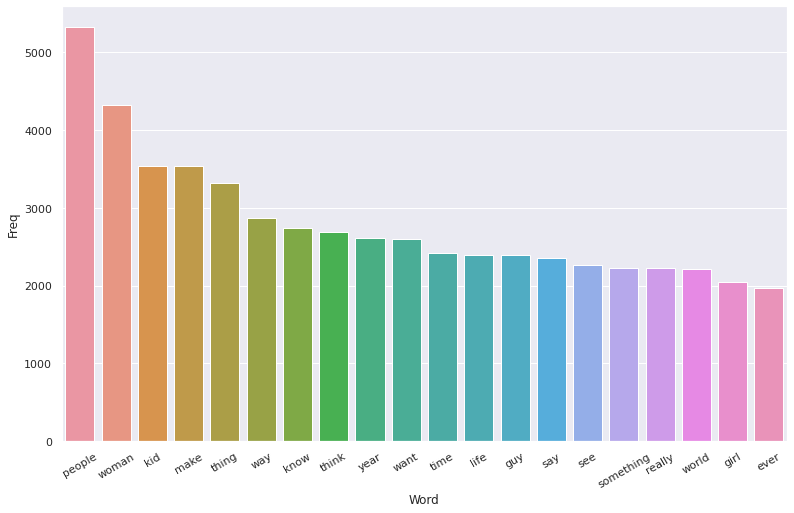
\includegraphics[scale=.3]{unigram_headline.png}
\caption{Unigram For Headline}
\end{figure} 

\begin{figure}[h]
\centering
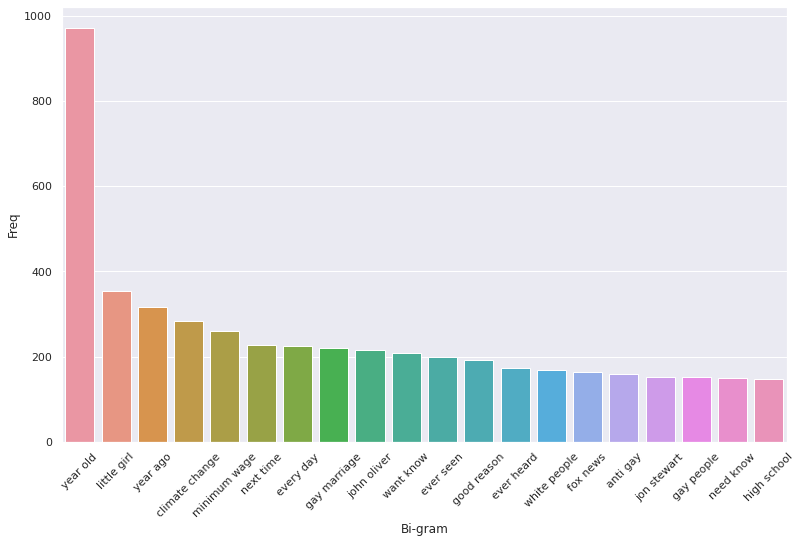
\includegraphics[scale=.3]{bigram_headline.png}
\caption{Bigram For Headline}
\end{figure} 

\begin{figure}[h]
\centering
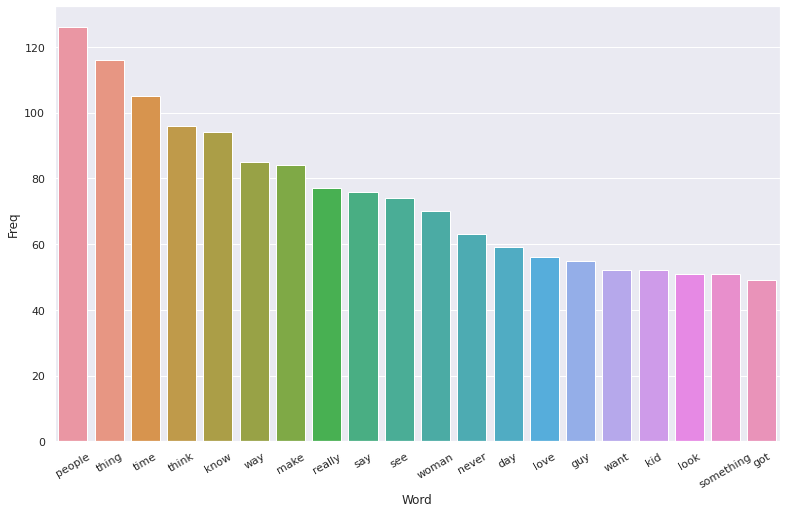
\includegraphics[scale=.3]{unigram_shared_text.png}
\caption{Unigram For Shared Text}
\end{figure} 

\vspace*{5em}
\subsection{Using Random Forest and SVM For Predict Metrics}
With this data,  we can start looking at models to use to predict the metrics that we want.  For classification, we decided to use a Support Vector Machine in order to predict the winner. Instead of using all 14 features, we filtered which features to use using the feature selection code from the scikit-learn library. The 3 features that were output were the number of characters in the headline, average word length in the headline, and number of capitalized characters in the headline. We used Support Vector Machines with a Radial Basis Function Kernel to classify new data as winners or not. Since this was a binary classification problem with non-linear data, we wanted to reduce the dimensionality of the problem by using a kernel. That is, we wanted to solve the following problem: 
\begin{align*}
\min_{\vb w, b} \frac{1}{2}\vert \vert \vb K(x, x') \cdot w \vert \vert^2 + C\sum_{i=1}^{k} \xi_{i} \\
\quad \textrm{s.t} \quad  y^{(i)}(\vb w^T \vb x_{i} + b) \geq 1 - \xi_{i} \\
\quad \textrm{and} \quad \xi_{i} \geq 0
\end{align*}
where $K(x, x') = exp( \frac{\vert x - x' \vert}{2\sigma^2})$.  Our Support Vector Machine model yielded a 92.4\% accuracy.  For predicting click to impressions ratio,  we decided to run Random Forest in order to predict the clicks to impressions ratio. Instead of using all 14 features, we filtered which features to use using the feature selection code from the scikit-learn library.  The 3 features that were output were the number of characters in the headline, average word length in the headline, and number of capitalized characters in the headline. This was quite surprising, as it did not include any of the “clickbait word” features, which we thought would play a big part in affecting clicks.Since our data was non-linear, we decided to opt for the Random Forest classifier since it is usually good at fitting non-linear datasets by using multiple decision tree classifiers and using averaging to improve predictive accuracy and control over-fitting.  The graphs for each feature and their predicted feature can be seen below.  Our Random Forest model yielded a 95\% accuracy.

\begin{figure}[h]
\centering
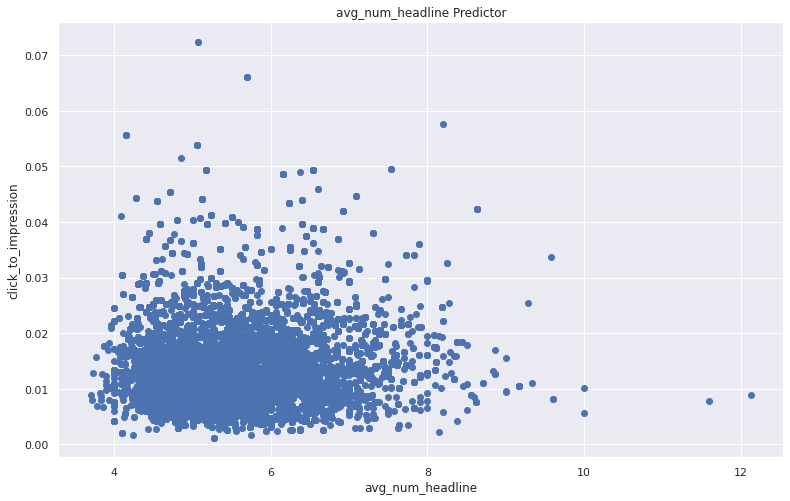
\includegraphics[scale=.3]{avg_num_headline_predict.png}
\caption{Average Number Headline Predicted Graph}
\end{figure} 

\begin{figure}[h]
\centering
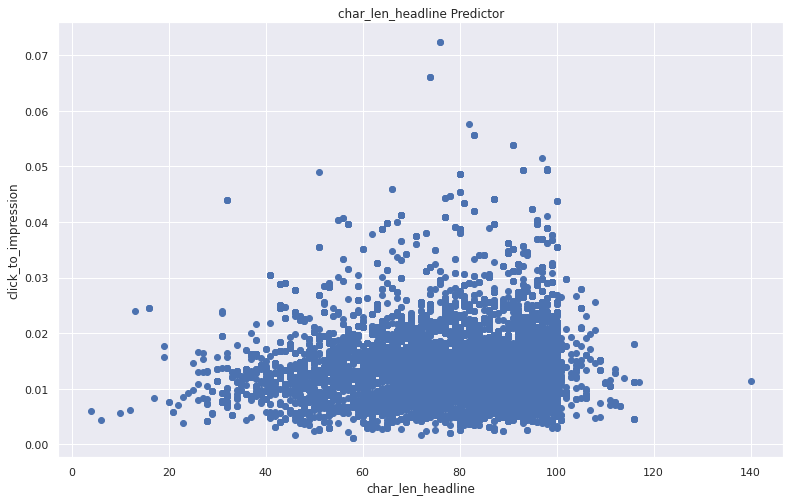
\includegraphics[scale=.3]{char_len_headline_predict.png}
\caption{Character Len Headline Predicted Graph}
\end{figure} 

\begin{figure}[h]
\centering
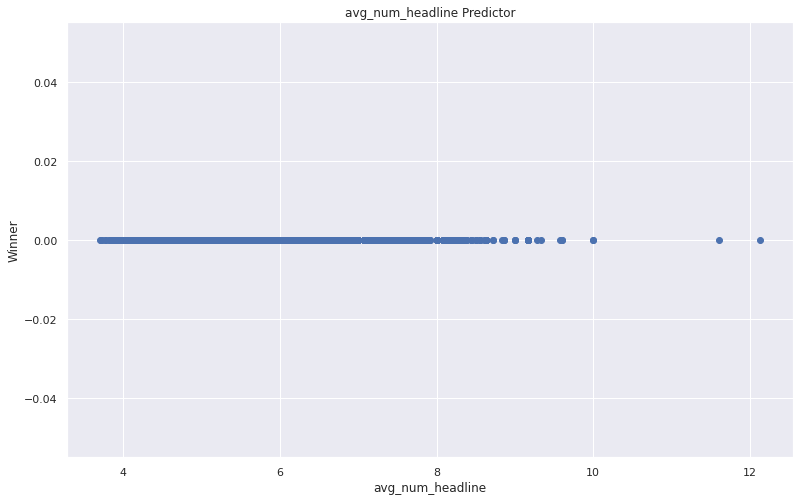
\includegraphics[scale=.3]{avg_num_headline_predictor_svm.png}
\caption{Average Number Headline Predicted SVM Graph}
\end{figure} 

\begin{figure}[h]
\centering
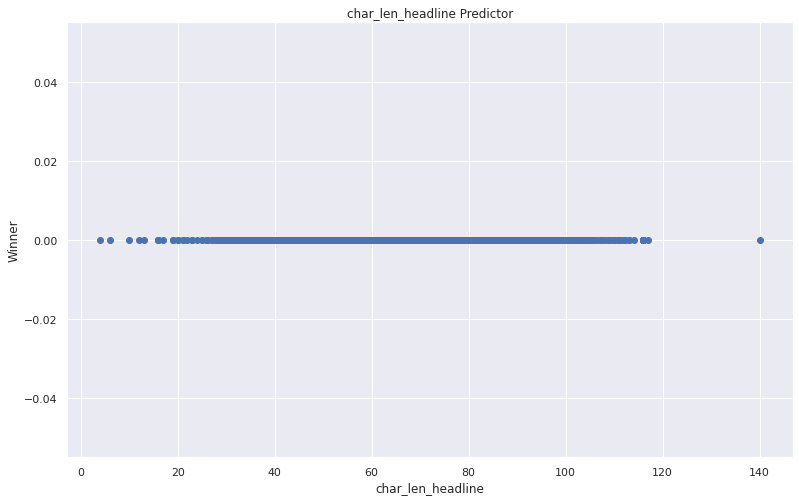
\includegraphics[scale=.3]{char_len_headline_predictor_svm.png}
\caption{Character Len Headline Predicted SVM Graph}
\end{figure} 

\begin{figure}[h]
\centering
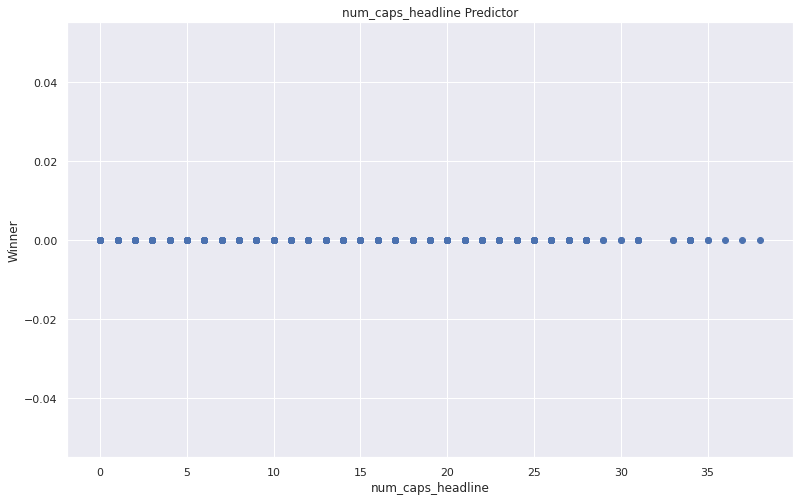
\includegraphics[scale=.3]{num_caps_headline_predictor_svm.png}
\caption{Number of Capitalized Letter Headline Predicted SVM Graph}
\end{figure} 
\vspace{12em}
\subsection{What We Learned}
It was interesting to see that after feature filtering for the Random Forest and SVM models, none of the “clickbait word” features were selected, which was surprising because we thought the “clickbait words” would play a large part in affecting clicks. It was also interesting to see that none of the shared text features were selected, because we assumed articles would have a large amount of shares, causing the shared text to affect the clicks.  According to the Random Forest model,  the optimal number of characters in a headline is 60-100 characters, with an average word length of 6 characters and 15-20 capitalized characters. We expected that a lot of capital letters would cause an increase in the click-to-impression ratio, but we were surprised to find out that headlines with more characters are more likely to get more clicks than shorter headlines.  According to the Support Vector Machine model,  having less words in the headline and thus less characters in the headline tends to yield winning packages.  Furthermore,  having between 0 and 20 capitalized letters in the headline also tends to yield winning packages. 

\end{document}